%\section{Preliminary}\label{sec:preliminary}
\section{Markov Decision Process}\label{sec:markov-decision-process}
\paragraph A Markov decision process (MDP) is a tuple $(S, A, P, R, \gamma)$, where: $S$ is a set of states. $A$ is a set of actions. $P(s'|s, a)$ is the probability of transitioning from state $s$ to state $s'$ when action $a$ is taken.
$R(s, a)$ is the reward received when taking action $a$ in state $s$. $\gamma \in [0, 1)$ is a discount factor that determines the importance of future rewards.
The MDP definition can be interpreted as follows:
\begin{itemize}
    \item The state $s$ represents the current state of the environment.
    \item The action $a$ represents the agent's decision in the current state.
    \item The transition probability $P(s'|s, a)$ represents the probability of the environment transitioning to state $s'$ after the agent takes action $a$ in state $s$.
    \item The reward $R(s, a)$ represents the amount of reward the agent receives after taking action $a$ in state $s$.
    \item The discount factor $\gamma$ represents how much the agent values future rewards relative to immediate rewards.
\end{itemize}
Decentralized Partially Observable Markov Decision Processes (Dec-POMDPs) are a class of MARL problems where multiple agents collectively aim to maximize a global objective function while facing uncertainty in a partially observable environment.

\subsection{Elements of Dec-POMDPs:}\label{subsec:elements-of-dec-pomdps:}
\begin{enumerate}
    \item \textbf{Agents:} Dec-POMDPs involve multiple agents denoted by index $i \in \{1, 2, \ldots, N\}$, each with its own local observation space $O_i$ and action set $A_i$. The agents interact with the environment and communicate with each other to make coordinated decisions.
    \item \textbf{States:} The environment's underlying state is not directly observable. Instead, each agent $i$ receives partial, private observations $o_i$ that provide probabilistic information about the true state. The state space is denoted as $S$.
    \item \textbf{Observations:} Each agent's observation $o_i$ is a partial and noisy representation of the global state. Observations are generated based on the current state $s$ and the agent's local observation function denoted as $O_i(s)$.
    \item \textbf{Actions:} Agents take actions $a_i$ based on their local observations and communication with other agents. The joint action of all agents affects the evolution of the underlying state. The joint action of all agents is denoted as $\mathbf{a} = (a_1, a_2, \ldots, a_N)$.
    \item \textbf{Transition Model:} The transition model $P(s' | s, \mathbf{a})$ describes the probability distribution over next states $s'$ given the current state $s$ and joint actions of all agents $\mathbf{a}$.
    \item \textbf{Observation Model:} The observation model $P(o_i | s)$ describes the probability distribution over observations $o_i$ given the current state $s$ for agent $i$.
    \item \textbf{Global Objective Function:} The goal of the agents is to optimize a global objective function $J(\mathbf{a})$ that captures the overall mission or task. This objective function depends on the collective actions of all agents and may involve cooperation and coordination.

\end{enumerate}

\section{Gaussian Distribution}\label{sec:gaussian-distribution}
The Gaussian distribution~\Cref{fig:guassian-distribution}, also known as the normal distribution, is a continuous probability distribution widely used to model random variables in various real-world scenarios. It is characterized by its mean $\mu$ and variance $\sigma^2$. The probability density function (PDF) of a Gaussian distribution is given by:

\begin{equation}
    f(x | \mu, \sigma^2) = \frac{1}{\sqrt{2\pi\sigma^2}} e^{-\frac{(x-\mu)^2}{2\sigma^2}},\label{eq:equation}
\end{equation}

where $x$ is a random variable, $\mu$ is the mean (expected value), and $\sigma^2$ is the variance.

The Gaussian distribution is symmetric around its mean, and its shape is determined by the variance. When the variance is small, the distribution is more concentrated around the mean, while a larger variance leads to a wider distribution.
\begin{figure}[!h]
    \centering
    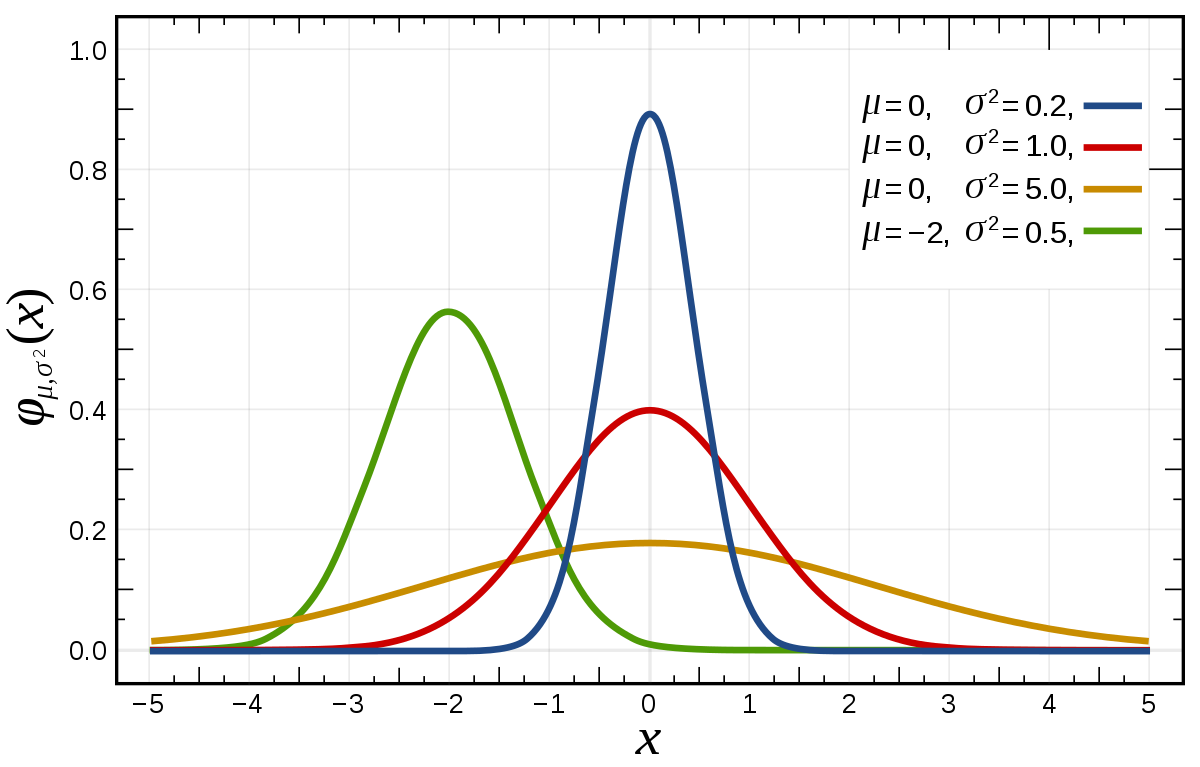
\includegraphics[width=12cm]{assets/normal}
    \caption{Normal Distribution}\label{fig:guassian-distribution}
\end{figure}

\section{Policy Gradient Method with Gaussian Approximation:}\label{sec:policy-gradient-method-with-gaussian-approximation:}
In RL, the policy gradient method is a popular approach to learning the policy of an agent in a continuous action space.
The policy gradient method directly optimizes the policy parameters to maximize the expected cumulative reward.

\subsection{Parameterized Policy}\label{subsec:parameterized-policy}
To handle continuous actions, the policy is often parameterized as a Gaussian distribution with a mean vector $\boldsymbol{\mu}$ and a variance vector $\boldsymbol{\sigma}^2$, or alternatively, using the standard deviation $\boldsymbol{\sigma}$. The policy function is defined as:

\begin{equation}
    \pi_{\boldsymbol{\theta}}(a | s) = \mathcal{N}(\boldsymbol{\mu}(s; \boldsymbol{\theta}), \text{diag}(\boldsymbol{\sigma}(s; \boldsymbol{\theta}))),\label{eq:equation2}
\end{equation}

where $\pi_{\boldsymbol{\theta}}(a | s)$ is the policy function with parameters $\boldsymbol{\theta}$, and $\text{diag}(\cdot)$ extracts the diagonal elements to form a diagonal covariance matrix.

\subsection{Prediction of Mean Using Neural Network}\label{subsec:prediction-of-mean-using-neural-network}
In practice, the mean $\boldsymbol{\mu}(s; \boldsymbol{\theta})$ is often predicted using a neural network with state $s$ as input and the policy parameters $\boldsymbol{\theta}$ as weights.
The neural network learns to map states to action means, allowing the agent to approximate actions based on observations from the environment.

\subsection{Adjusting Standard Deviation Over Time}\label{subsec:adjusting-standard-deviation-over-time}
During the training process, the standard deviation $\boldsymbol{\sigma}(s; \boldsymbol{\theta})$ can be adjusted over time.
It is often initialized with some initial value and then decayed towards a minimum value~\cite{capasso2021endtoend},\cite{sutton2018reinforcement},\cite{mnih2015humanlevel}.
This adjustment allows the agent to explore more at the beginning of training (high uncertainty) and become more confident in its actions as training progresses (low uncertainty).

\section{Beta Distribution}\label{sec:beta-distribution}
The Beta distribution~\Cref{fig:beta-distribution} is a continuous probability distribution defined on the interval [0, 1].
It is commonly used to model random variables that represent probabilities or proportions.
The Beta distribution is parameterized by two shape parameters, denoted as $\alpha$ and $\beta$, which control the shape of the distribution. The PDF of the Beta distribution is given by:

\begin{equation}
    f(x | \alpha, \beta) = \frac{1}{B(\alpha, \beta)} x^{\alpha - 1}(1 - x)^{\beta - 1},\label{eq:equation4}
\end{equation}

where $x$ is a random variable, $\alpha$ and $\beta$ are the shape parameters, and $B(\alpha, \beta)$ is the Beta function:

\begin{equation}
    B(\alpha, \beta) = \frac{\Gamma(\alpha) \Gamma(\beta)}{\Gamma(\alpha + \beta)},\label{eq:equation3}
\end{equation}

where $\Gamma(\cdot)$ is the gamma function.

The Beta distribution is asymmetric and its shape is determined by the values of $\alpha$ and $\beta$. When both $\alpha$ and $\beta$ are greater than 1, the distribution is unimodal and skewed.
The mode of the distribution is at $\frac{\alpha - 1}{\alpha + \beta - 2}$.

\begin{figure}[h!]
    \centering
    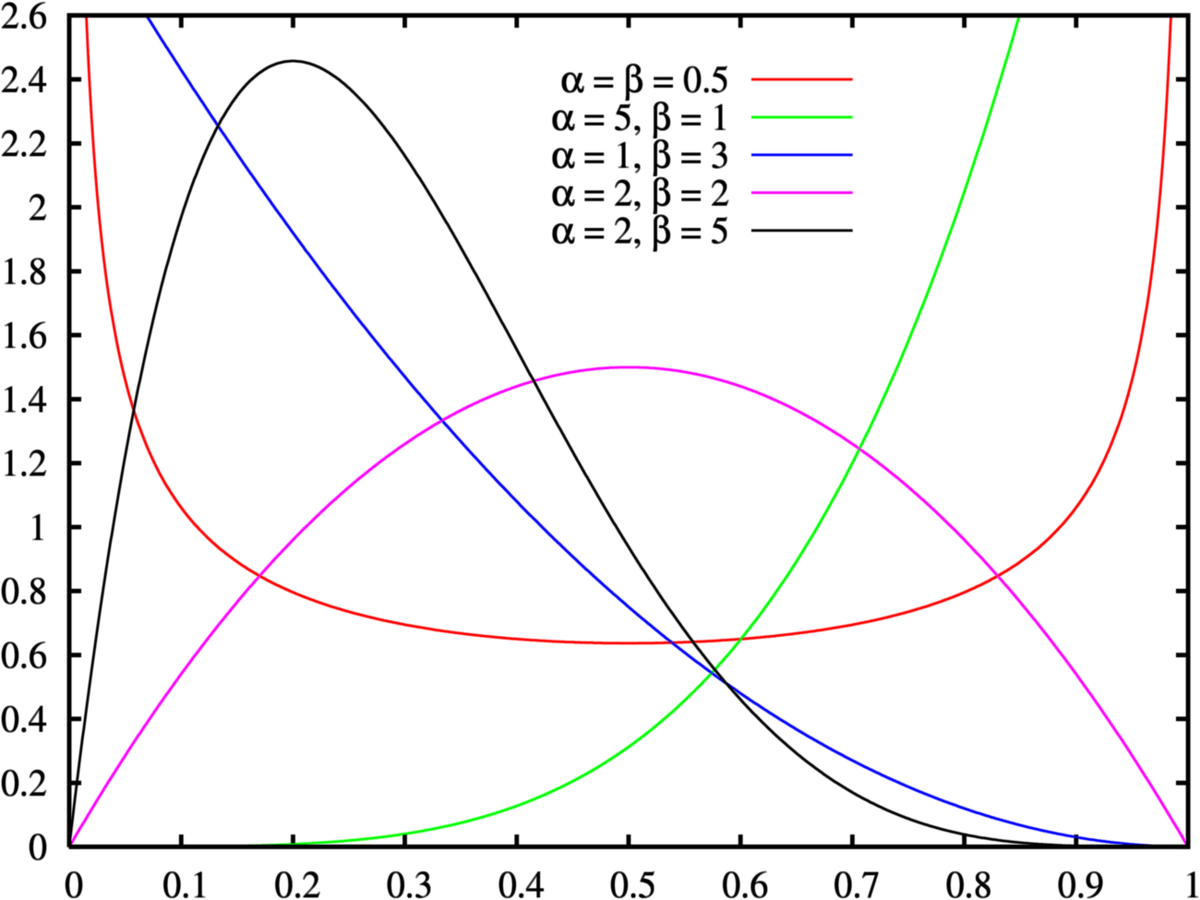
\includegraphics[width=12cm]{assets/beta}
    \caption{Beta Distribution}\label{fig:beta-distribution}
\end{figure}

\section{Policy Gradient Method with Beta Distribution:}\label{sec:policy-gradient-method-with-beta-distribution:}
In the policy gradient method for RL, the policy is often parameterized as a Beta distribution to handle continuous actions within the range [0, 1].

\subsection{Predicting Alpha and Beta Values from Neural Network:}\label{subsec:predicting-alpha-and-beta-values-from-neural-network:}
To approximate the Beta distribution for policy generation, a neural network is used to predict the $\alpha$ and $\beta$ parameters.
The neural network takes the state $s$ as input and produces the $\alpha$ and $\beta$ values as output.
These values are then used to define the Beta distribution for sampling actions.

\subsection{Interpretation of 1 - $\alpha$ and 1 - $\beta$:}\label{subsec:interpretation-of-1---$alpha$-and-1---$beta$:}
The $\alpha$ and $\beta$ values can be interpreted as counts of successes and failures, respectively.
Specifically, if $\alpha > 1$ and $\beta > 1$, then $\alpha - 1$ and $\beta - 1$ can be thought of as the number of successes and failures, respectively.
This interpretation is useful when modeling probabilities or proportions in the context of the policy gradient method.

\section{Beta Policy}\label{sec:beta-policy}
\paragraph We propose a straightforward neural network architecture, specifically a Multilayer Perceptron (MLP), with 2 hidden layers each having a size of 256 neurons as we can see in~\cref{fig:beta-policy}. This neural network is then divided into two separate channels, each having a hidden layer with 256 neurons. These channels are designed to predict values for steering angle and acceleration, respectively, in order to control the vehicle.

The implementation of the neural network is carried out using PyTorch~\cite{paszke2019pytorch}, a popular deep learning library. The input to the network consists of ego states, which include relevant information about the vehicle in relation to its environment, such as velocity, checkpoint positions, time, and distance to the destination. Additionally, LiDAR data from the left, right, and front sides of the vehicle is collected and fed into the network. LiDAR is a sensing technology used in many AVs, and its utilization allows the proposed algorithm to be easily adapted and applied in real-world scenarios.
\begin{figure}[h!]
    \centering
    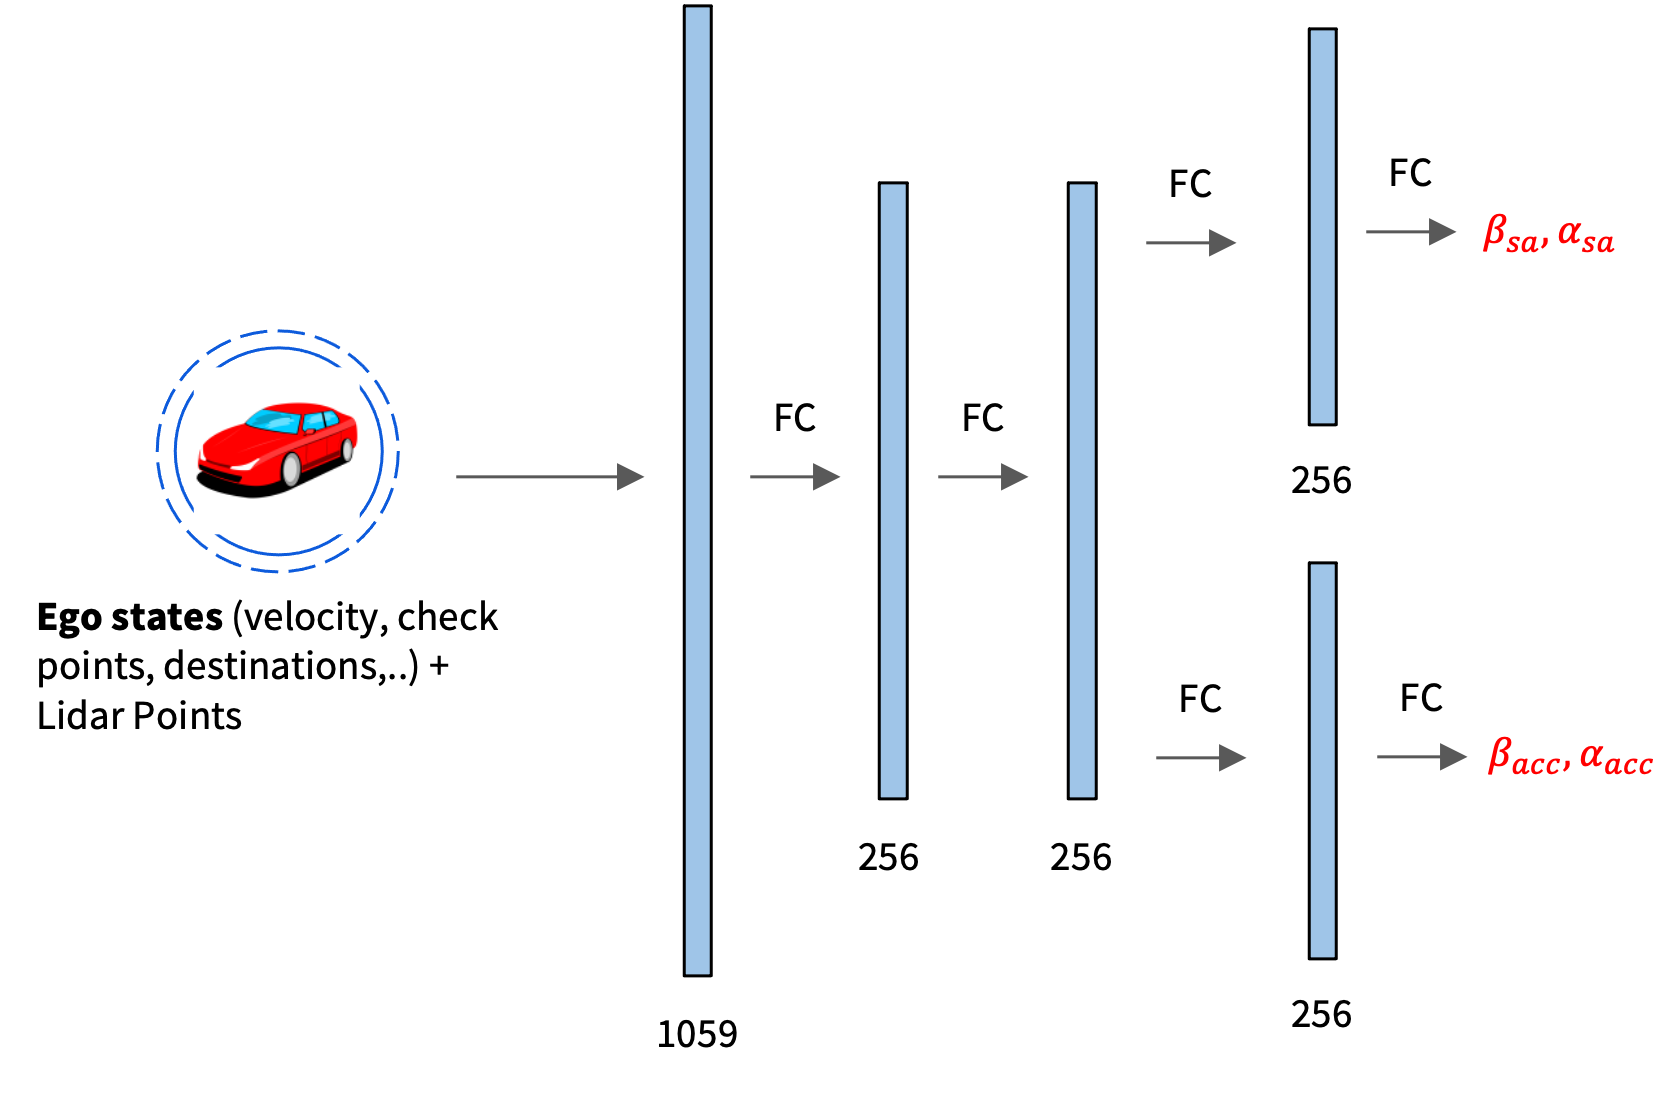
\includegraphics[width=12cm]{assets/beta_policy}
    \caption{Beta Policy}\label{fig:beta-policy}
\end{figure}

The final layer that output these values uses softplus
activation function and 1 is added to make sure that the output
is always positive. The final layer is $f(x) = 1 + \log (1 +
e^x)$ . As the environment accepts action with $a = [sa,acc]^T=[-1,1]^2$, the output from Beta's PDF is then mapped with the following equation:
\begin{equation}
    sa = 2h(\beta_{sa}, \alpha_{sa}) - 1\label{eq:equation5}
\end{equation}
\begin{equation}
    acc = 2h(\beta_{acc}, \alpha_{acc}) - 1\label{eq:equation6}
\end{equation}

where $h(\beta, \alpha)$ is the mean of the Beta distribution with parameters $\beta$ and $\alpha$, $sa$ stands for steering angle, and $acc$ stands for acceleration.
It should be noted that we only consider the case where $\alpha > 1$ and $\beta > 1$.

\section{Advantage Function (Experience Sharing)}\label{sec:advantage-function}
\paragraph The advantage function is a key component of the policy gradient method.
It is used to estimate the advantage of taking an action $a$ in state $s$ over taking an action sampled from the policy $\pi$ in state $s$.
The advantage function is defined as:
\begin{equation}
    A^{\pi_{\theta_{k}}}(s_{t},s_{t+1}, A_{j}, A_{j+1}, R_{G}) = R_{G} +  Q(s_{t+1}, A_{j+1}) - Q(s_{t}, A_{j})\label{eq:equation7}
\end{equation}
where $R_{G}$ is the global reward defined as $R_{G} = \frac{1}{k} \sum_{i=0}^{k}R_{k} $
whose $k$ is the individual reward calculated by Monte Carlo Method~\cite{sutton2018reinforcement}.  $Q(\star)$ is the critics part which is popularized by Asynchronous Advantage Actor Critic (A3C)~\cite{mnih2016asynchronous} and also adopted by PPO~\cite{schulman2017proximal}
, $Q(s_{t}, A_{j})$ is the Q-value of taking action $A_{j}$ in state $s_{t}$, and $A_{j+1}$ is the action sampled from the policy $\pi$ in state $s_{t+1}$.
\begin{figure}[!h]
    \centering
    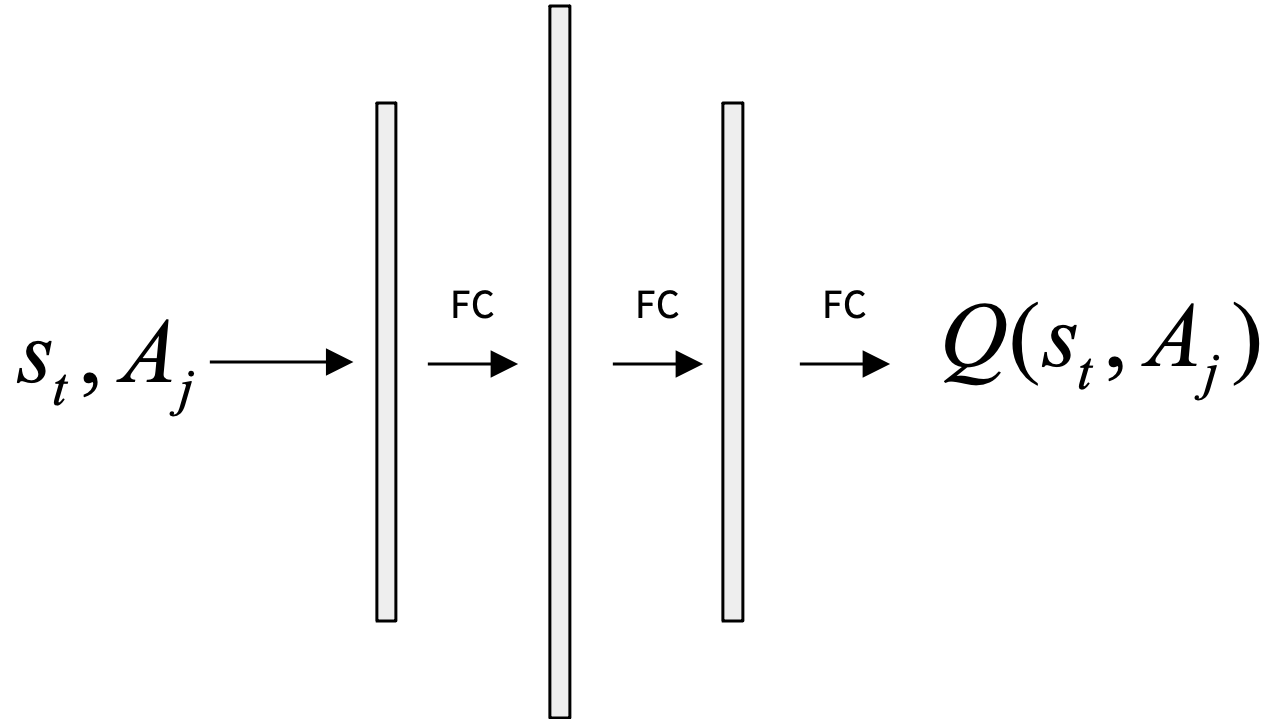
\includegraphics[width=10cm]{assets/advantage_fun}
    \caption{$Q$ value Approximator (Critics)}\label{fig:figure4}
\end{figure}

\section{Objective Function}\label{sec:objective-function}
\paragraph The objective function is used to optimize the policy parameters $\theta$. The goal of the agent is to maximize the culminative reward over time by updating the parameterized policy with:
\begin{equation}
    \theta_{k+1} = \arg\max_{\theta} \frac{1}{|D_{k}|T} \sum_{\tau\in D_{k}}^{} \sum_{t=1}^{T} \min (\frac{\pi_{\theta}(a_{t}|s_{t})}{\pi_{\theta_{k}}(a_{t}|s_{t})} A^{\pi_{\theta_{k}}}, g(\epsilon, A^{\pi_{\theta_{k}}}))\label{eq:equation8}
\end{equation}
where $D_{k}$ is the set of trajectories collected by the agent at iteration $k$, $T$ is the length of the trajectory, $\pi_{\theta}$ is the policy parameterized by $\theta$, and $g(\epsilon, A^{\pi_{\theta_{k}}})$ is the clipped surrogate objective function defined as:
\begin{equation}
    g(\epsilon, A^{\pi_{\theta_{k}}}) = \begin{cases}
        (1 + \epsilon) A^{\pi_{\theta_{k}}} & \text{if } A^{\pi_{\theta_{k}}} \geq 0 \\
        (1 - \epsilon) A^{\pi_{\theta_{k}}} & \text{otherwise}
    \end{cases}\label{eq:equation9}
\end{equation}

\section{Centralized Training and Decentralized Execution(CTDE)}\label{sec:centralized-training-and-decentralized-execution}
CTDE starts with several agents being placed in the
environment. The agents are allowed to run for several
predefined steps (2000 timestamps in our case). In the process,
samples are collected in a rollout buffer, the buffer then
performs some preprocessing tasks such as arranging data and
splitting data into experience batches.
Those baches are then
fed into the central agent's actor-critics network to update the
policy by calculating loss and through back propagation.
The updated policy is then distributed back to the individual agent.
The cycle repeats until the reward feedback converges.
\begin{figure}[!h]
    \centering
    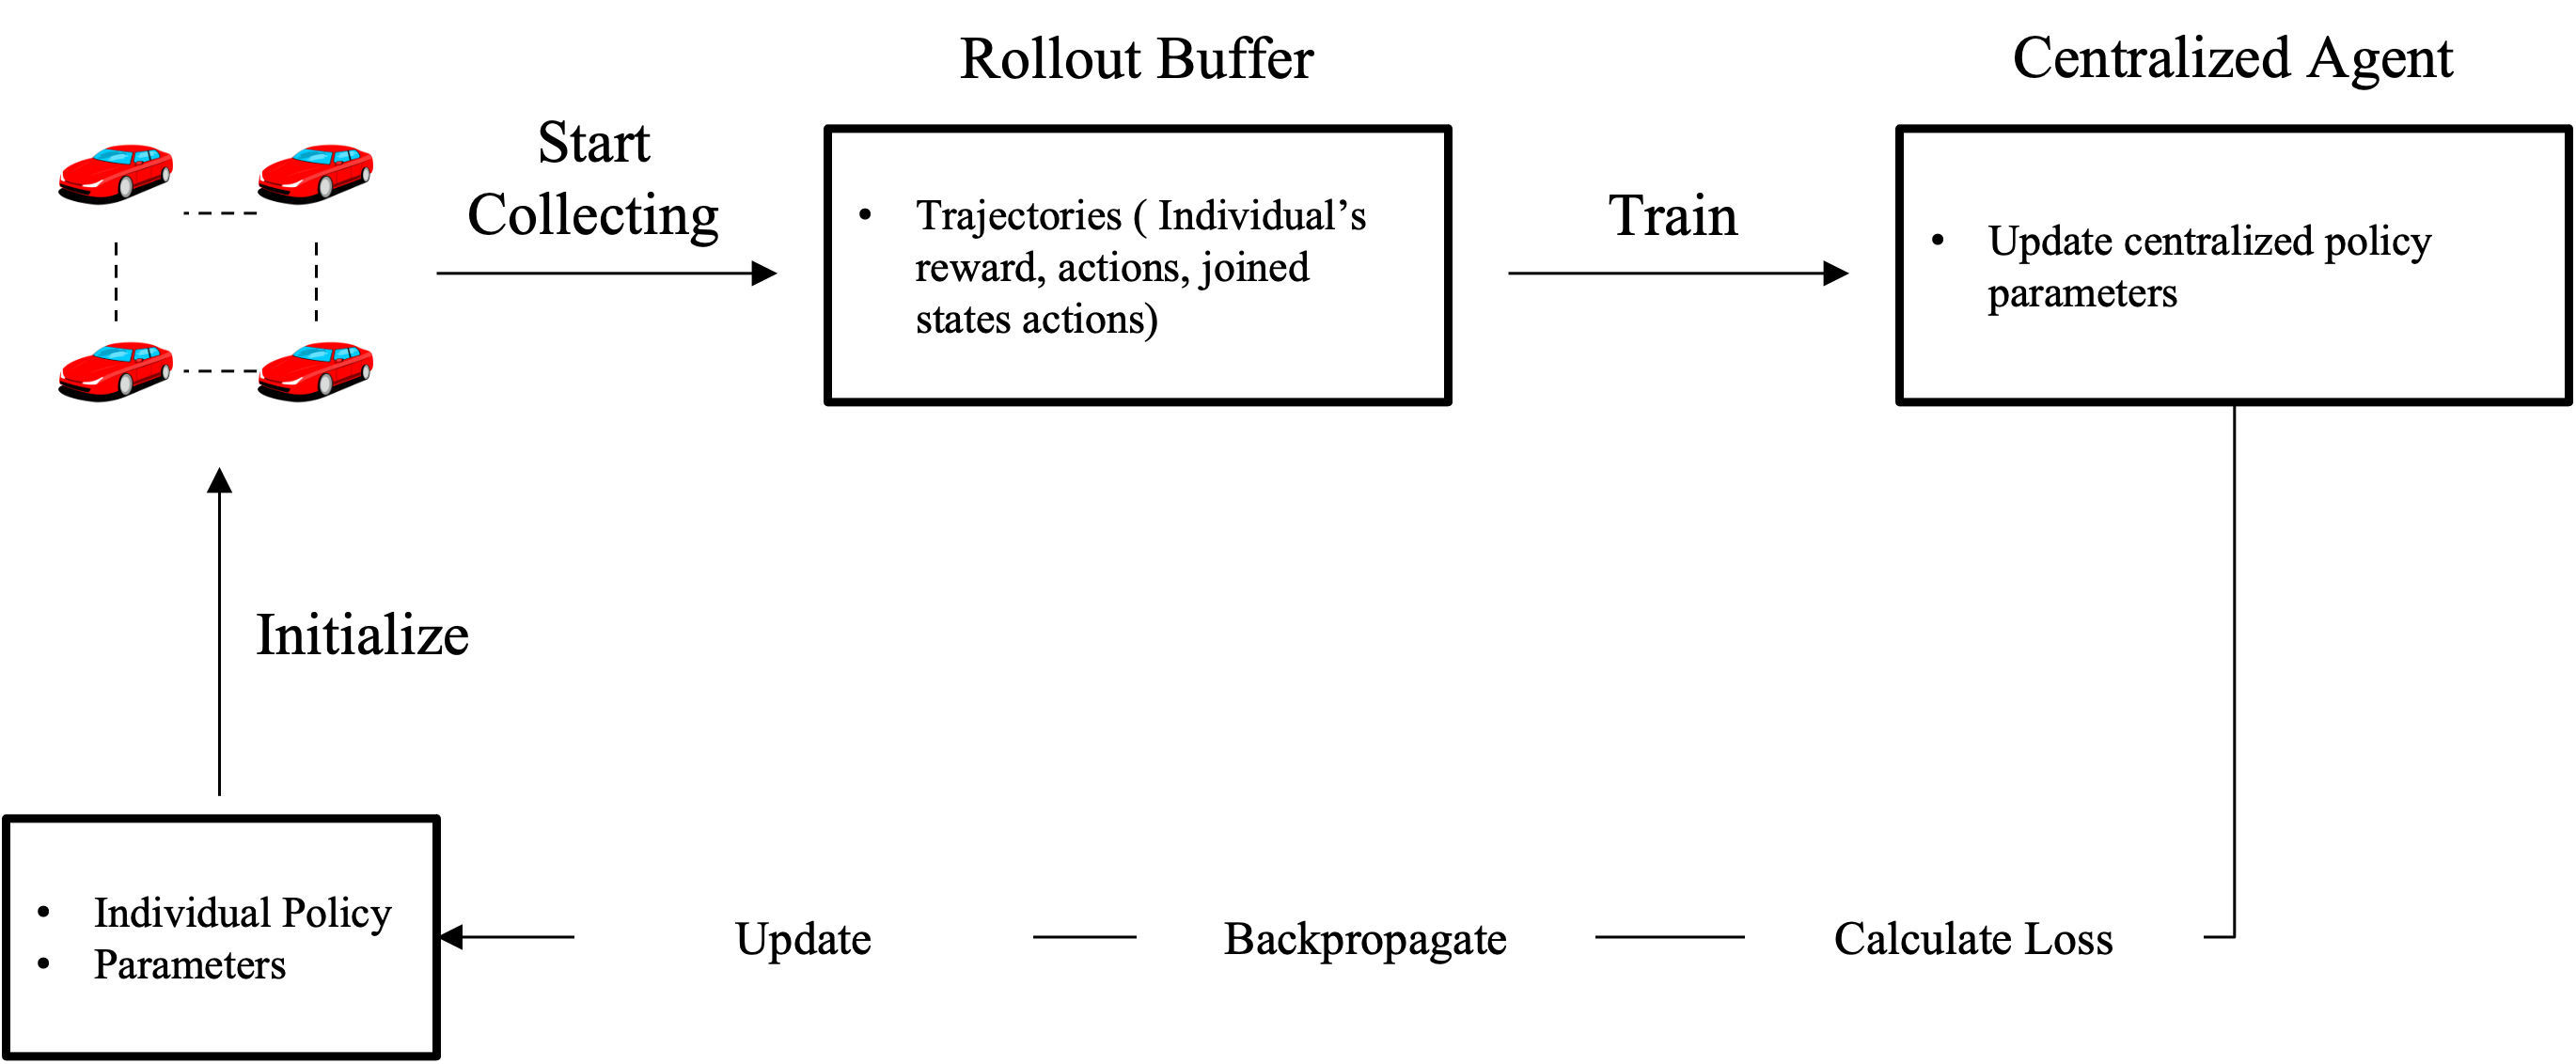
\includegraphics[width=14cm]{assets/clde}
    \caption{Centralized Training and Decentralized Execution}\label{fig:figure5}
\end{figure}